\documentclass[12pt,a4paper]{report}

\usepackage[MeX]{polski} 
\usepackage[utf8]{inputenc} %Kodowanie znaków, zależne od systemu
\usepackage[T1]{fontenc} 	%Poprawne składanie polskich czcionek

\usepackage{textcomp}

%Pakiet służący do wypisywania adresów stron internetowych
\usepackage{url}

%Pakiety do grafiki
\usepackage{graphicx}
\usepackage{subfigure}
\usepackage{ccaption}
\usepackage{psfrag}

%Pakiety dodające dużo dodatkowych poleceń matematycznych
\usepackage{amsmath}
\usepackage{amsfonts}

%Pakiety wspomagające i poprawiające składanie tabel
\usepackage{supertabular}
\usepackage{array}
\usepackage{tabularx}
\usepackage{hhline}
\usepackage{multirow}
\renewcommand{\arraystretch}{1.5}

%Pakiet służący do definiowania interlnii w części dokumentu
\usepackage{setspace}	

%Pakiet wstawia wcięcie na początku akapitu po section, subsection
\usepackage{indentfirst}

%Pakiet umożliwia dodanie interaktywności do standardowych odwołań
\usepackage{hyperref}

\setlength{\parindent}{1.25cm}	%Wcięcie akapitu

%%%Nowa sttrona tytułowa
\usepackage[top=2cm, bottom=2cm, left=3cm, right=3cm]{geometry}
%Pozwala używać '@'
\makeatletter 
%Polecenie pomocnicze - pionowa linia, szeroka na 4 mm
\newcommand{\linia}{\rule{\linewidth}{0.4mm}}

\renewcommand{\maketitle}{\begin{titlepage}
    \vspace*{1cm}
    
    \begin{center}\small
    Politechnika Wrocławska\\
    Wydział Elektroniki\\
    Katedra Automatyki, Mechatroniki i Systemów Sterowania
    \end{center}
    
    \vspace{3cm}
    
    \noindent\linia
    \begin{center}
      \Huge \textsc{\@title} \\
      \Large Projekt
    \end{center}
    \linia
    
    \vspace{0.5cm}
    
    \begin{flushright}
    \begin{minipage}{6.5cm}
    \textit{\small Autorzy:}\\
    \normalsize \textsc{Sebastian Kowalewski, 184145} \par
    \normalsize \textsc{Bartłomiej Kozdraś, 184095} \par
    \normalsize \textsc{Karol Rungo, 184128} \par
    \vspace{0.5cm}
    \textit{\small Prowadzący:}\\
    \normalsize \textsc{Dr inż. Jarosław Pempera} \par
    \vspace{0.5cm}
    \textit{\small Termin:}\\
    \normalsize \textsc{Wt TN $11^{15}$-$13^{00}$} \par
    \end{minipage}
    \end{flushright}    
     
    \vspace*{\stretch{6}}
    
    \begin{center}
    \@date
    \end{center}
    
    \newpage
	\thispagestyle{empty}
	\mbox{}
  \end{titlepage}%
}
%Znowu nie pozwala używać '@'
\makeatother
%%%Koniec

\title{Optymalizacja dyskretnych procesów produkcyjnych}
\date{31 marca 2015}

\begin{document}
\maketitle	
\tableofcontents

%\newpage
%\thispagestyle{empty}
%\mbox{}

\chapter{Wstęp}

\section{Przedstawienie problemu}
Przedstawiony w~projekcie problem dotyczy serwisanta technicznego pracującego w~firmie telekomunikacyjnej, do którego obowiązków należy serwis stacji bazowych (ang.~\textit{Base Transceiver Station}, BTS), które odgrywają podstawową rolę w~systemach łączności. Głównym zagadnieniem jest wybór konkretnych miejscowości,w~których znajdują się BTSy, a~następnie odwiedzenie ich w~takiej kolejności, aby zminimalizować czas lub koszt podróży, ewentualnie odległość pomiędzy miastami. W~zagadnieniach optymalizacyjnych problem taki jest znany jako problem komiwojażera.

Projekt zakłada stworzenie aplikacji graficznej, do której dostęp będę mieli serwisanci oraz administratorzy. Administrator może edytować bazę danych poprzez dodanie lub usuwanie stacji bazowych oraz serwisantów. Serwisant korzysta z~aplikacji wybierając miasta, które musi odwiedzić. Aplikacja na podstawie wskazanych miast wylicza najbardziej korzystną drogę oraz przedstawia jej przebieg na mapie. 

\section{Problem komiwojażera}
Problem komiwojażera (ang.~\textit{Travelling salesman problem}) w~dobry sposób opisuje następujące pytanie: znając listę miast i odległość pomiędzy każdą parą miast, jaka jest najkrótsza droga, aby odwiedzić dokładnie każde z~nich jeden raz, a~następnie wrócić do miasta początkowego? TSP jest problemem NP--trudnym stosowanym w~optymalizacji kombinatorycznej, a~także ważnym zagadnieniem w~badaniach operacyjnych i~algorytmice \cite{TSP_Wiki}. 

Nie ulega wątpliwości, że problem komiwojażera w~bardzo dobry sposób ilustruje przedstawiony problem serwisanta, który musi w~ramach swojej pracy odwiedzić wskazane stacje bazowe. W~ten sposób w~niniejszym projekcie zaprezentowano rzeczywisty problem, który może zostać rozwiązany za pomocą zagadnienia szeroko znanego w~nauce.

Najczęściej spotykaną wersją problemu komiwojażera jest minimalizacja przebytej drogi. Oczywiście długość drogi nie jest jedynym dopuszczalnym parametrem. Można założyć, że znana jest cena lub czas podróży. W~takim przypadku rozwiązanie problemu polega na znalezieniu najtańszej bądź najszybszej drogi, który musi przebyć komiwojażer.

Problem komiwojażera często przedstawiany jest za pomocą grafów. Okazuje się, że teoria grafów dostarcza rozwiązań, które w~dobry sposób reprezentują omawiane zagadnienie. Wierzchołki grafów mogą pełnić rolę miast, natomiast krawędzie są połączeniami pomiędzy parą konkretnych miejscowości. Waga przypisana każdej z~krawędzi może opisywać parametr (odległość, koszt lub czas) charakteryzujący połączenie pomiędzy miastami. 

TSP jest problemem NP--trudnym. Oznacza to, że istniejące algorytmy rozwiązujące ten problem mają bardzo niekorzystną, wykładniczą złożoność obliczeniową. Dokładne algorytmy działają dla bardzo małej liczby miast, najlepiej w~sytuacji gdy graf, nie jest grafem zupełnym. Istnieje jednak spora grupa algorytmów przybliżonych. W~takich przypadkach nie otrzymuje się rozwiązania optymalnego, ale często uzyskany przybliżony rezultat jest zadowalający. 

\chapter{Zastosowane narzędzia, oprogramowanie i algorytmy}

\section{Microsoft Visual Studio 2013}
Microsoft Visual Studio 2013 jest zintegrowanym środowiskiem programistycznym (ang.~\textit{Integrated Development Environment}, IDE), które
umożliwia programiście tworzenie samodzielnych aplikacji. Produkt ten wspiera platformę .NET i~język C Sharp, dlatego też został zastosowany w~ramach realizowanego projektu. Ponadto możliwe jest tworzenie aplikacji dla systemów desktopowych --- klasycznych, jak i~wykorzystujących interfejs Modern UI\footnote{Modern UI (ang.~\textit{Modern User Interface}), to wcześniejsza wersja Microsoft design language, co jest wewnętrzną nazwą kodową dla języka projektowania firmy Microsoft. Interfejs Modern UI jest wykorzystywany, np.~w Windowsie 8 czy Windows Phone.}. Co istotne zapewnia nowoczesne i~zaawansowane elementy interfejsu WPF\footnote{WPF (ang.~\textit{Windows Presentation Foundation}), to nazwa silnika graficznego i~API bazującego na .NET.}, co wydaje się być szczególne istotne przy zastosowaniu Microsoft Blend.

Vicsual Studio zawiera edytor kodu, który wspiera IntelliSense\footnote{IntelliSense jest formą automatycznego uzupełniania zawartą w~niektórych środowiskach programistycznych, co pozwala skrócić proces pisania kodu, redukując pomyłki stylistyczne, literówki, etc.} oraz mechanizmy refaktoryzacji kodu. Zintegrowany ze środowiskiem debugger, pozwala programiście na badanie przebiegu wykonywania kodu i~obserwację dowolnej używanej zmiennej. Poprzez udostępnienie designera do tworzenia aplikacji Windows Forms, skonstruowanie odpowiedniego interfejsu graficznego jest intuicyjne i~relatywnie proste. Zastosowanie ma tutaj metoda "przeciągnij--upuść", co znacznie skraca czas tworzenia oprogramowania.

Istotną rolę odgrywa również fakt, że programista otrzymuje dużą swobodę podczas tworzenia oprogramowania z~wykorzystaniem omawianego IDE. Visual Studio praktycznie na każdym poziomie aplikacji można rozszerzać za pomocą dodatków, a~kod można wzbogacać o~dołączone biblioteki.

\section{Język C Sharp i platforma .NET}
C Sharp (C\#), to obiektowy język programowania zaprojektowany dla firmy Microsoft. Łączy w~sobie najlepsze cechy takich języków jak C++ czy Java. Co istotne program napisany w~tym języku kompilowany jest do specjalnego kodu pośredniego wykonywanego w~środowisku uruchomieniowym, jakim jest, np.~platforma .NET. Nie jest możliwe wykonanie skompilowanego programu przez system operacyjny nieposiadający takiego środowiska.

Wśród głównych cech języka warto wymienić:
\begin{itemize}
  \item obiektowość,
  \item Garbage Collector --- mechanizm zajmujący się gospodarowaniem pamięcią, zwalniający programistę z~obowiązku zwalniania zaalokowanej pamięci,
  \item type ogólne (generyczne) --- mechanizm zbliżony do szablonów w~C++,
  \item obsługa zdarzeń i~delegatów.
\end{itemize}

Platforma programistyczna .NET Framework  została opracowana i~udostępniona w~2002~r. przez firmę Microsoft. Obejmuje środowisko uruchomieniowe oraz biblioteki klas, które służą dostarczeniu aplikacjom odpowiednich funkcjonalności. Głównym zadaniem platformy jest zarządzanie różnymi elementami systemu, m.~in. kodem i/lub pamięcią. Platforma .NET nie jest ściśle związana z~jednym językiem programowania. Jest wspierana, np.~przez C++, C~Sharp czy Visual Basic. Co ciekawe w~2014~r. Microsoft zapowiedział udostępnienie .NET na zasadach Open Source  (licencja MIT).

Język C~Sharp w~połączeniu z~platformą .NET umożliwia proste tworzenie
rozbudowanych i~wydajnych aplikacji. Bogate biblioteki klas umożliwiają tworzenie programów z~graficznym interfejsem użytkownika (GUI), konsolowych, bazodanowych czy internetowych.

\section{SQL Server Management Studio 2008}
SQL Server Management Studio, to rozbudowana aplikacja, służąca do zarządzania bazami danych Microsoft. Narzędzie wyposażone jest w~prosty, graficzny interfejs i~posiada wiele użytecznych kreatorów ułatwiających pracę z~bazą danych, m.~in.: konfigurację oraz administrowanie instancjami SQL Server.

Korzystanie z~omawianego oprogramowania zapewnia szereg funkcjonalności do tworzenia, edytowania i~zarządzania bazą danych. Użyta w~projekcie wersja SQL Server Management Studio 2008 Express charakteryzuje się darmową licencją. 

\section{Technologia LINQ}
LINQ (ang.~\textit{Language INtegrated Query}), to część technologii platformy  dot NET. Jest technologią zaptań związanych z~językiem programowania. Zapewnia wygodny dostęp do danych. Jako, że stanowi warstwę abstrakcji nad różnymi źródłami danych, może obsługiwać:

\begin{itemize}
  \item bazę danych SQL,
  \item dokument XML,
  \item zwykły obiekt (pod warunkiem, że implementuje interfejs IEnumerable<T>).
\end{itemize}

Jako swój wynik zapytanie LINQ zwraca „kolejkę” obiektów typu ogólnego. Sama technologia oferuje wiele operatorów i~funkcji do tworzenia bardzo skomplikowanych zapytań. Składnia języka jest relatywnie prosta i~bardzo przypomina składnię znaną z~SQL.

\section{Microsoft Blend}
Microsoft Blend\footnote{Wcześniej znany jako Microsoft Expression Blend.}, to narzędzie opracowane przez firmę Microsoft służące do tworzenia zaawansowanych graficznych interfejsów aplikacji internetowych, a~także desktopowych. Jest edytorem opartym na XAML (ang.~\textit{eXtensible Application Markup Language})\footnote{XAML jest językiem opisu interfejsu użytkownika wykorzystywanym m.~in.~w~technologii Windows Presentation Foundation.}. Z~jego pomocą projektuje się interfejsy dla WPF oraz Microsoft Silverlight\footnote{Microsoft Silverlight, to technologia internetowa, dzięki której możliwe jest wyświetlenie treści multimedialnych używając do tego przeglądarki internetowej.}. Do działania wymaga koniecznie platformy .NET.

W 2012 r., wraz z~wydaniem Microsoft Windows 8, zmieniono nazwę na Blend for Visual Studio". Od tego momentu program wydawany jest wraz z~oprogramowaniem Microsotf Visual Studio. Należy jednak zaznaczyć, że nie jest podstawowym wyposażeniem wszystkich wersji wspomnianego IDE.

\section{GMap.NET}
GMap.NET, to wieloplatformowe, darmowe, opensource'owe narzędzie działające pod kontrolą .NET. Umożliwia wykonywania wielu operacji na mapach:

\begin{itemize}
  \item Google,
  \item Yahoo!,
  \item Bing,
  \item OviMap,
  \item WikiMapia,
  \item i innych \cite{GMap}.
\end{itemize}

Wśród zapewnionych funkcji możliwe jest rysowanie drogi oraz znalezienie lokacji za pomocą współrzędnych geograficznych lub podania jej nazwy. Narzędzie, to odgrywa ważną rolę w~projekcie, gdyż pozwala na graficzne przedstawienie trasy, którą musi pokonać serwisant.

\section{Algorytm}

\subsection{Przedstawienie problemu na grafach}
Problem komiwojażera został przybliżony w~pierwszym rozdziale. W~terminologii grafów należy dokonać założeń, że miasta są wierzchołkami grafu, natomiast trasy pomiędzy nimi --- krawędziami. Waga krawędzi może być liczbą opisującą różne pojęcia, w~zależności od tego, co jest celem optymalizacji. Może odpowiadać, np.: czasowi podróży, kosztom przejazdu, odległości pomiędzy miastami. Trasa komiwojażera jest cyklem, który przechodzi przez każdy wierzchołek grafu dokładnie jeden raz (z~wyjątkiem pierwszego --- tutaj cykl się zaczyna i~kończy). Taki cykl określa się mianem cyklu hamiltonowskiego. 

Znalezienie właściwego cyklu Hamiltona metodą przeglądu zupełnego jest zadaniem trudnym obliczeniowo. Na rys.~2.1 przedstawiono graf zupełny (każdy wierzchołek połączony z~każdym) o~dziesięciu wierzchołkach. Liczba różnych cykli hamiltonowskich jest równa $(n - 1)!$, gdzie $n$ odpowiada liczbie wierzchołków, co prowadzi do złożoności obliczeniowej $O(n!)$.

\begin{figure}[!bht]
\centering
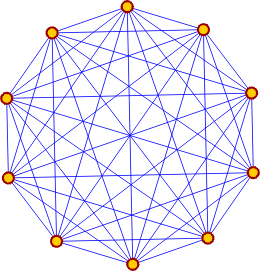
\includegraphics[scale=0.5]{Pictures/CompleteGraph.png}
\label{fig: CompleteGraph}
\caption{Graf zupełny dla dziesięciu wierzchołków}{Źródło: \url{http://edu.i-lo.tarnow.pl/inf/alg/001_search/0140.php}}
\end{figure}

Przykładowy cykl hamiltonowski zaprezentowano na rys.~2.2. Dla każdego znalezionego cyklu należałoby policzyć sumę wag i~zapamiętać cykl, dla którego suma ta jest najmniejsza. Grafy, które odzwierciedlają rzeczywiste połączenia pomiędzy miastami nie są zupełne, gdyż nieekonomiczne byłoby budowanie osobnych dróg pomiędzy każdą parą miast. Nie zmienia to jednak faktu, że problem nadal posiada klasę złożoności obliczeniowej $O(n!)$.

\begin{figure}[!bht]
\centering
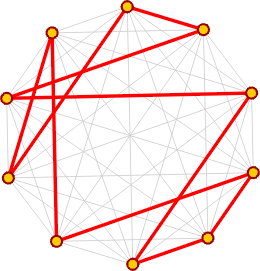
\includegraphics[scale=0.5]{Pictures/ExampleHamiltonCycle.png}
\label{fig: ExampleHamiltonCycle}
\caption{Przykładowy cykl Hamiltona w grafie o dziesięciu wierzchołkach}{Źródło: \url{http://edu.i-lo.tarnow.pl/inf/alg/001_search/0140.php}}
\end{figure}

Istnieją algorytmy zwracające rozwiązanie przybliżone w~czasie wielomianowym, lecz zazwyczaj są one bardzo zaawansowane. Przy założeniu jednak, że liczba krawędzi nie jest duża, co wydaje się być bardzo sensowne, gdyż serwisant raczej nie odwiedzi dużej liczby miast w~krótkim okresie czasu, a~graf nie jest grafem zupełnym, to rozwiązanie problemu komiwojażera można uzyskać prostym algorytmem. Algorytm ten polega na wyznaczeniu wszystkich cyklów Hamiltona, policzenia sumy wag krawędzi i~zwróceniu cyklu o~najmniejszej sumie wag. Co najważniejsze otrzymany w~ten sposób wynik jest optymalny, a~nie przybliżony. 

\subsection{Algorytm rozwiązujący problem komiwojażera}
Zastosowany algorytm rozwiązuje problem komiwojażera dla małych grafów. Uwzględniając jednak zagadnienie znalezienie najkrótszej drogi pomiędzy stacjami bazowymi przez serwisanta wydaje się być to sensowne, ponieważ pracownik nie jest w~stanie odwiedzić zbyt dużej liczby BTSów w~krótkim czasie. 

Zaproponowany pomysł opiera się na rekurencyjnej procedurze \cite{TSP_Tarnow}:

\begin{center}
\verb+TSP(n, graph, v ,vo, d, dH, S, SH, visited)+,
\end{center}
gdzie:

\begin{itemize}
  \item \verb+n+ --- liczba wierzchołków w grafie,
  \item \verb+graph+ --- zadany w~dowolnie wybrany sposób. Definicja grafu powinna udostępniać wagi krawędzi (w~projekcie zrealizowany poprzez macierz sąsiedztwa),
  \item \verb+v+ --- wierzchołek bieżący,
  \item \verb+vo+ --- wierzchołek startowy,
  \item \verb+d+ --- suma wag krawędzi cyklu hamiltonowskiego,
  \item \verb+dH+ --- pomocnicza suma wag krawędzi,
  \item \verb+S+ --- stos wierzchołków,
  \item \verb+SH+ --- pomocniczy stos wierzchołków,
  \item \verb+visisted+ --- \verb+n+--elementowa tablica logiczna odwiedzin.
\end{itemize}
Wyjściem procedury jest \verb+S+ --- stos zawierający numery kolejnych wierzchołków cyklu Hamiltona o~najmniejszej sumie wag krawędzi (stos pusty, gdy cykl Hamiltona nie istnieje) oraz \verb+d+ --- suma wag krawędzi cyklu hamiltonowskiego. Wyróżnia się jeszcze wierzchołek pomocniczy \verb+u+.

Lista kroków algorytmu głównego prezentuje się następująco:

\begin{itemize}
  \item[1] Utwórz i wyzeruj \verb+visisted+, \verb+S+, \verb+SH+.
  \item[2] \verb+d+ $\leftarrow \infty$, \verb+dH+ $\leftarrow 0$ (początkowa suma największa z~możliwych).
  \item[3] \verb+TSP(vo)+ (wyszukiwanie cyklu Hamiltona od wierzchołka startowego).
  \item[4] Jeśli \verb+S.empty() = false+, to pisz \verb+S+ i \verb+d+, inaczej pisz "Brak cyklu Hamiltona".
  \item[5] Zakończ
\end{itemize}

Natomiast lista kroków procedury rekurencyjnej jest znacznie dłuższa i~została przedstawiona poniżej:

\begin{itemize}
  \item[1] \verb+SH.push(v)+ (odwiedzony wierzchołek dopisany do ścieżki).
  \item[2] Jeśli \verb+SH+ nie zawiera \verb+n+ wierzchołków, to idź do 10 (brak ścieżki Hamiltona).
  \item[3] Jeśli nie istnieje krawędź z \verb+v+ do \verb+vo+, to idź do 17 (brak cyklu Hamiltona).
  \item[4] \verb+dH+ $\leftarrow$ \verb+dH+ + waga krawędzi z \verb+v+ do \verb+vo+ (uwzględnienie w sumie ostatniej wagi).
  \item[5] Jeśli \verb+dH+ $\geq$ \verb+d+, to idź do 8 (znaleziony cykl jest gorszy od bieżącego).
  \item[6] \verb+d+ $\leftarrow$ \verb+dH+ (zapamiętanie sumy wag cyklu).
  \item[7] Skopiuj stos \verb+SH+ do stosu \verb+S+ (zapamiętanie cyklu Hamiltona).
  \item[8] \verb+dH+ $\leftarrow$ \verb+dH+ - waga krawędzi z \verb+v+ do \verb+vo+ (usunięcie ostatniej wagi z sumy).
  \item[9] Idź do 17.
  \item[10] \verb+visisted(v)+ $\leftarrow$ \verb+true+ (wierzchołek zaznaczony jako odwiedzony).
  \item[11] Dla każdego sąsiada \verb+u+ wierzchołka \verb+v+ wykonuj 12...15 (lista sąsiedztwa).
  \item[12] Jeśli \verb+visisted(v) = true+, to przejdź do 11 (omijanie wierzchołków odwiedzonych).
  \item[13] \verb+dH+ $\leftarrow$ \verb+dH+ + waga krawędzi z \verb+v+ do \verb+u+ (nowa suma wag krawędzi cyklu).
  \item[14] \verb+TSP(n, graph, u, vo, d, dH, S, SH, visited)+ (rekurencyjne poszukiwanie cyklu).
  \item[15] \verb+dH+ $\leftarrow$ \verb+dH+ - waga krawędzi z \verb+v+ do \verb+u+ (usunięcie wagi krawędzi z sumy).
  \item[16] \verb+visisted(v)+ $\leftarrow$ \verb+false+ (zwolnienie bieżącego wierzchołka).
  \item[17] \verb+SH.pop()+ (usunięcie bieżącego wierzchołka ze ścieżki).
  \item[18] Zakończ.
\end{itemize}

\chapter{Opis aplikacji}

\section{Baza danych}
Baza danych została stworzona w~środowisku SQL Server Management Studio 2008, które opisane została we wcześniejszym rozdziale. Poszczególne tabele, które są użyte w~zaprojektowanej aplikacji, zostały przedstawiono na rys.~\ref{fig: Database}.

\begin{figure}[!bht]
\centering
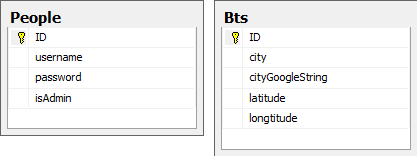
\includegraphics[scale=1]{Pictures/Database.png}
\label{fig: Database}
\caption{Tabele w bazie danych}{Źródło: opracowanie własne}
\end{figure}

Tabela \textit{People} zawiera loginy i~hasła wszystkich użytkowników korzystających z~aplikacji. Podczas logowania do programu, następuje sprawdzenie czy w~bazie danych istnieje użytkownik o~podanym loginie i~haśle przy pomocy zapytania zrealizowanego w~technologii LINQ. Tabela nie jest powiązana relację z~tabelą \textit{Bts}. Dodanie nowego użytkownika do systemu możliwe jest tylko z~poziomu administratora. Za sprawdzenie czy czy zalogowany użytkownik posiada kompetencje pozwalające na zarządzanie bazą odpowiada zmienna bitowa \verb+isAdmin+. Działanie takie ma na celu zabezpieczenie przed umyślnym dodaniem nowego użytkownika bez wiedzy administratora.

\textit{Bts} jest tabelą, która zawiera lokalizacje konkretnych stacji bazowych. Nie jest powiązana żadną relacją z~tabelą \textit{People}. BTS jest identyfikowany poprzez przypisane mu miasto, długość oraz szerokość geograficzną. Zmienna \verb+cityGoogleString+ jest niezbędna do prawidłowego zastosowania narzędzia GMap.NET. Tylko użytkownik o~statusie administratora może dodawać lub usuwać stacje bazowe z~bazy danych.

Połączenie aplikacji okienkowej z~bazą danych odbywa się za pomocą klasy \verb+DataContext+. W~celu uaktywnienia połączenia należy stworzyć obiekt tej klasy i~w~specjalnie wygenerowanym pliku wybrać tabele z~bazy, na których aplikacja będzie operować. 

\section{Okna aplikacji}
Aplikacja została wyposażona w~wiele okien użytkownika. Każde z~nich pełni osobną funkcjonalność. Wszystkie okna wyposażone zostały w~różnego rodzaju kontrolki, które pozwalają na interakcję z~operatorem. Rozmieszczenie elementów jest intuicyjne, a~przyciski zostały pokolorowane odpowiednim kolorem powodującym właściwe skojarzenia (czerwony --- usuń, zielony --- akceptuj).

Na rys.~3.2 przedstawiono okno logowania aplikacji. W~tym miejscu użytkownik powinien wpisać swój login oraz hasło, a jeżeli jest administratorem musi zaznaczyć także pole \textit{Admin}. Następnie po wciśnięciu przycisku \textit{Log in} zostanie przeniesiony, z~odpowiednimi uprawnieniami, do menu głównego programu. Naciśnięcie przycisku \textit{Info} powoduje wyświetlenie najważniejszych informacji na temat programu (autorzy, kurs oraz prowadzący).

\begin{figure}[!bht]
\centering
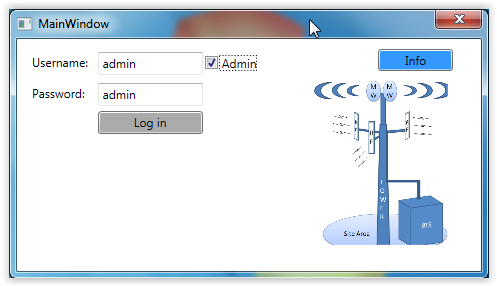
\includegraphics[scale=0.5]{Pictures/MainWindow.png}
\label{fig: MainWindow}
\caption{Okno logowania}{Źródło: opracowanie własne}
\end{figure}

Menu główne aplikacji została zaprezentowane na rys.~3.3. Warto zaznaczyć, że serwisant może kliknąć tylko i~wyłącznie przycisk \textit{Route planning}. Pozostałe możliwości są dostępne tylko dla użytkownika z~uprawnieniami administratora. Klikając odpowiednie przyciski można przejść kolejno do okna: zarządzania stacjami bazowymi, planowania drogi oraz zarządzania pracownikami.

\begin{figure}[!bht]
\centering
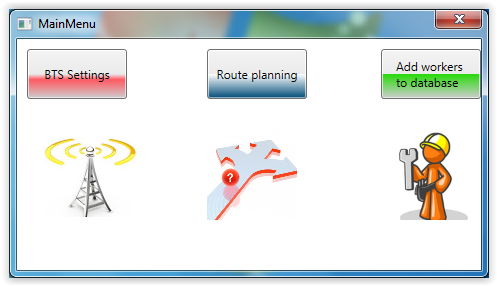
\includegraphics[scale=0.5]{Pictures/MainMenu.png}
\label{fig: MainMenu}
\caption{Menu główne programu}{Źródło: opracowanie własne}
\end{figure}

Okno zarządzania stacjami bazowymi (rys.~3.4) umożliwia dodane lub usuwanie miejscowości, w~których znajdują się BTSy. W~polu tekstowym obok etykiety \textit{City} należy wpisać nazwę miasta, którym zainteresowany jest użytkownik. Aplikacja obsługuje polskie znaki diakrytyczne. Następnie po wciśnięciu przycisku \textit{Search for location} w~tabeli poniżej zostaną wyświetlone odpowiednie lokacje. Zaznaczenie lokacji odbywa się poprzez naciśnięcie jej lewym przyciskiem myszy. Gdy miejscowość zostanie zaznaczona, można kliknąć na zielony przycisk \textit{Add location to database}, co spowoduje dodanie miasta do bazy danych. Analogicznie postępuje się w~przypadku usuwania lokacji. W~górnej tabeli należy zaznaczyć miejscowość, a~następnie kliknąć na czerwonym przycisku \textit{Delete selected BTS}. Należy zapamiętać, że można dodać oraz usunąć tylko jeden wiersz (aplikacja nie wspiera wielokrotnego jednorazowego dodawania oraz usuwania). Dostęp do omawianego okienko posiada tylko użytkownik o~statusie adminsitratora.

\begin{figure}[!bht]
\centering
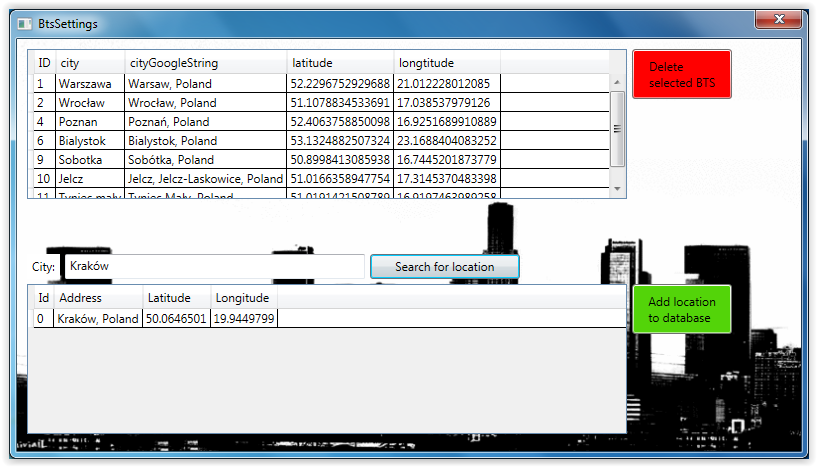
\includegraphics[scale=0.5]{Pictures/BtsSettings.png}
\label{fig: BtsSettings}
\caption{Okno zarządzania stacjami bazowymi}{Źródło: opracowanie własne}
\end{figure}

Do okna planowania drogi (rys.~3.5) dostęp mają zarówno serwisanci jak i~administratorzy. Obsługa jest bardzo intuicyjna. Zaznaczenie miasta w~tabeli po lewej stronie, a~następnie kliknięcie przycisku \textit{>>} powoduje jego przeniesienie to tabeli po prawej stronie. Miasta, które znajdują się w~tabeli po prawej stronie biorą udział w~ustalania optymalnej trasy, przy czym pierwsze miasto jest lokacją początkową. Miejscowość z~prawej tabeli można oczywiście przenieść do lewej poprzez zaznaczenie jej, a~następnie naciśnięcie przycisku \textit{<<}. Podobnie jak we wcześniejszych oknach, program umożliwia przeniesienie jednorazowo tylko jednego miasta. Kliknięcie przycisku \textit{Start planning!} spowoduje obliczenie optymalnej trasy i~narysowanie jej na mapie. Aby jednak zobaczyć wyrysowaną trasę należy wykonać operację przybliżenia/oddalenia na mapie.

\begin{figure}[!bht]
\centering
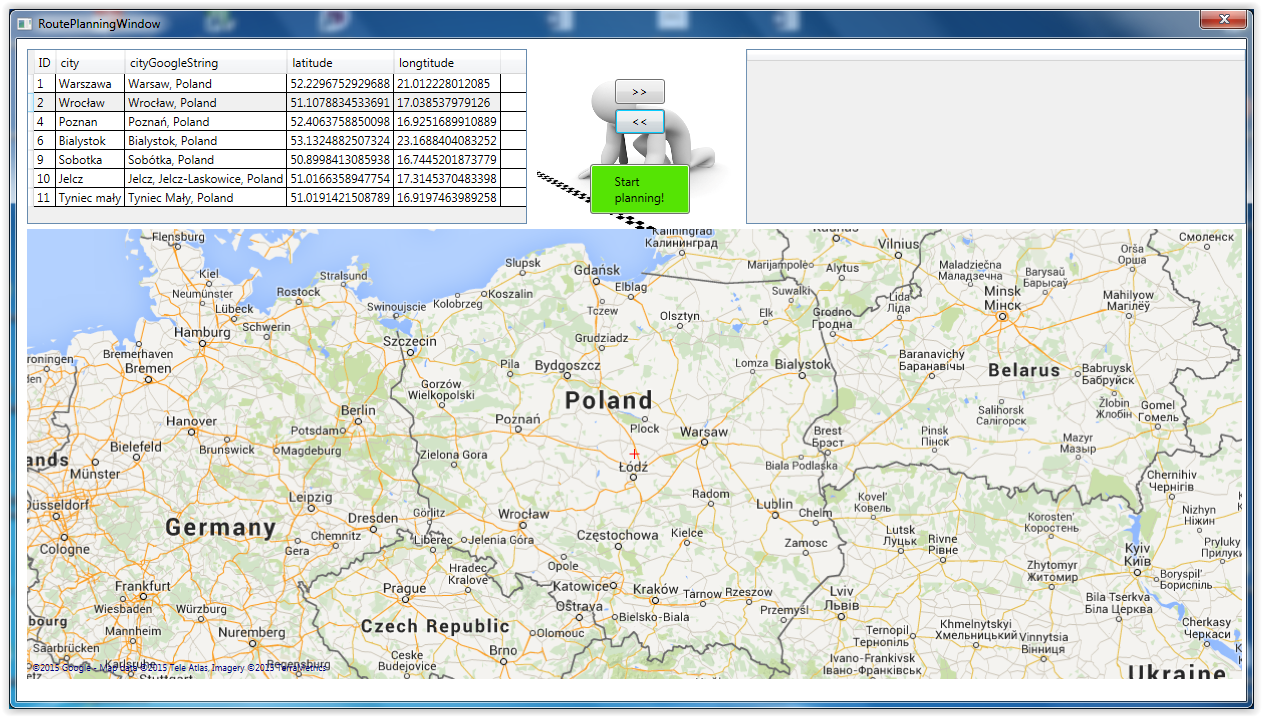
\includegraphics[scale=0.37]{Pictures/RoutePlanning.png}
\label{fig: RoutePlanning}
\caption{Okno planowania drogi}{Źródło: opracowanie własne}
\end{figure}

Ostatnie okno zostało przedstawiono na rys.~3.6. Umożliwia zarządzanie kadrą pracowniczą. Z~przyczyn oczywistych jest dostępne tylko dla użytkownika o~statusie administratora. Aby dodać serwisanta, bądź administratora, należy wpisać w~odpowiednie pola login oraz hasła, a~także zaznaczyć prawa dostępu (pole \textit{Is admin?}), a~następnie kliknąć przycisk \textit{Add user}. Usuwanie użytkownika odbywa się poprzez jego zaznaczenie w~tabeli, a~następnie naciśnięcie czerwonego przycisku \textit{Delete selected user}. Podobnie jak wcześniej można usunąć tylko jednego użytkownika przy jednym kliknięciu przycisku. 

\begin{figure}[!bht]
\centering
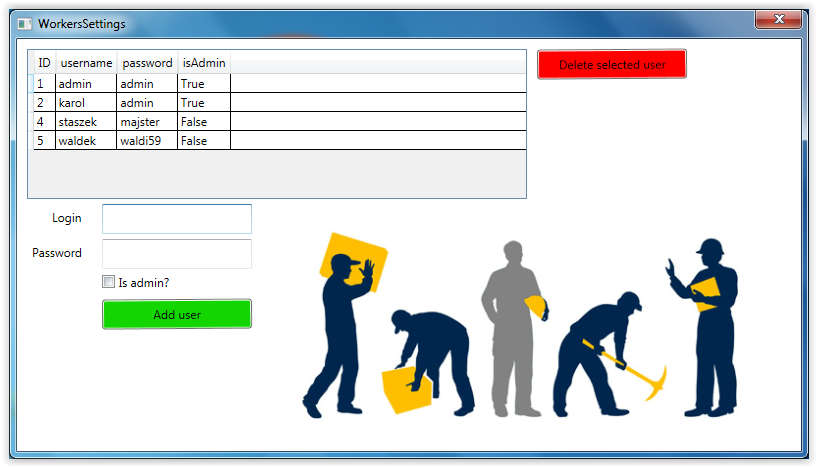
\includegraphics[scale=0.5]{Pictures/WorkerSettings.png}
\label{fig: WorkerSettings}
\caption{Okno zarządzania pracownikami}{Źródło: opracowanie własne}
\end{figure}

\chapter{Prezentacja działania programu}

W niniejszym rozdziale zaprezentowano przykładowe działanie programu. Starano się przedstawić jego funkcjonalność oraz zastosowanie. Opis został wzbogacony za pomocą zrzutów ekranu przedstawiających testowaną aplikację.

Ekranem, który wita użytkownika po uruchomienie aplikacji, jest okno logowania. Program dopuszcza obecność dwóch grup użytkowników: serwisantów, którzy mogą tylko planować drogę, oraz administratorów, którzy poza znajdowaniem optymalnej trasy posiadają także możliwość zarządzania użytkownikami oraz lokalizacją stacji bazowych.

Na rys.~4.1 przedstawiono nieudaną próbę logowania przez serwisanta, który zaznaczył jako aktywną opcję \textit{Admin}. Niestety pan Waldek nie posiada praw administratora, więc przy próbie wejścia do systemu otrzymał komunikat o~błędzie.

\begin{figure}[!bht]
\centering
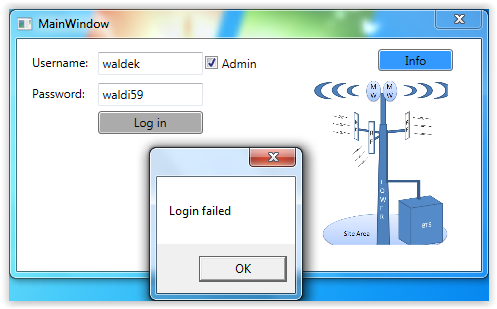
\includegraphics[scale=1]{Pictures/LoginFailedWaldek.png}
\label{fig: LoginFailedWaldek}
\caption{Błędne logowanie serwisanta}{Źródło: opracowanie własne}
\end{figure}

Podobna sytuacja może spotkać administratora. Została przedstawiona na rys.~4.2. Program nie pozwoli na zalogowanie użytkownika o~statusie administratora bez zaznaczonej funkcji \textit{Admin}. Za pomocą komunikatu o~błędzie przypomina o~tym, że odpowiednie pole musi zostać zaznaczone.

\begin{figure}[!bht]
\centering
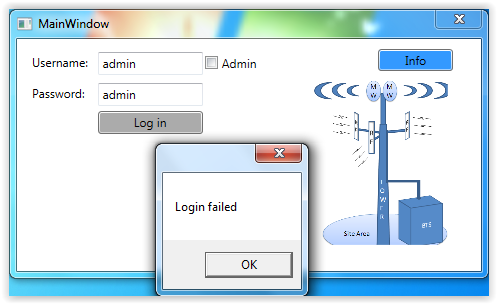
\includegraphics[scale=1]{Pictures/LoginFailedAdmin.png}
\label{fig: LoginFailedAdmin}
\caption{Błędne logowanie administratora}{Źródło: opracowanie własne}
\end{figure}
\newpage
Na rys.~4.3 przedstawiono prawidłowo przeprowadzoną próbę logowania. Administrator wpisał właściwy login oraz hasło, a~ponadto zaznaczył pole \textit{Admin}. W~ten sposób po kliknięciu przycisku \textit{Log in} zostanie on zalogowany do systemu.

\begin{figure}[!bht]
\centering
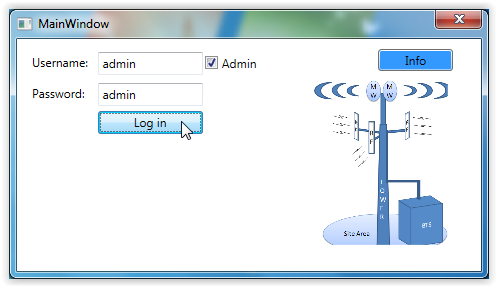
\includegraphics[scale=1]{Pictures/LoginAcceptAdmin.png}
\label{fig: LoginAcceptAdmin}
\caption{Logowanie administratora zakończone sukcesem}{Źródło: opracowanie własne}
\end{figure}

Okienko logowania posiada również przycisk \textit{Info}. Po jego kliknięciu pojawi się okienko informujące o~autorach aplikacji oraz podstawowych informacjach z~nią związanych (rys.~4.4).

\begin{figure}[!bht]
\centering
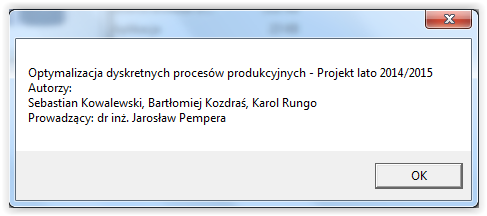
\includegraphics[scale=1]{Pictures/Authors.png}
\label{fig: Authors}
\caption{Okienko informacyjne programu}{Źródło: opracowanie własne}
\end{figure}
\newpage
Po prawidłowym przejściu procesu logowania oczom administratora ukaże się okienko głównego menu (rys.~4.5). Użytkownik o~statusie administratora, klikając odpowiedni przycisk, może wybrać jedną z~trzech akcji: zarządzania stacjami bazowymi, planowanie trasy, zarządzanie użytkownikami. Intuicyjny rysunek pod każdym z~nich przywodzi na myśl odpowiednie skojarzenia z~funkcjonalnością, która kryje się pod każdym przyciskiem. Powoduje to, że aplikacja jest prosta, intuicyjna i~przyjemna w~użyciu. 

\begin{figure}[!bht]
\centering
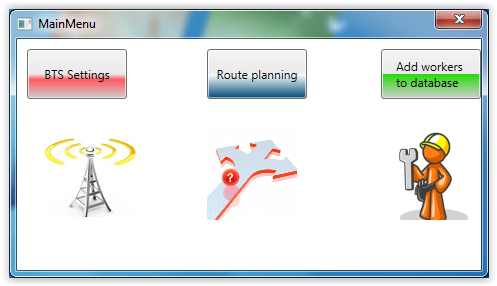
\includegraphics[scale=1]{Pictures/MainMenuAdmin.png}
\label{fig: MainMenuAdmin}
\caption{Funkcje dostępne w głównym menu dla administratora}{Źródło: opracowanie własne}
\end{figure}

Ekran głównego menu będzie wyglądał trochę inaczej, jeżeli zalogowanym użytkownikiem jest serwisant (rys.~4.6). Jego uprawnienia pozwalają tylko i~wyłącznie na planowanie drogi. Wydaje się być to sensownym rozwiązaniem, gdyż nie ma większego sensu, aby umożliwić pracownikowi dodawanie BTSów, których konserwacją zajmuje się firma, a~tym bardziej zapewnienie możliwości zarządzania innymi użytkownikami.

\begin{figure}[!bht]
\centering
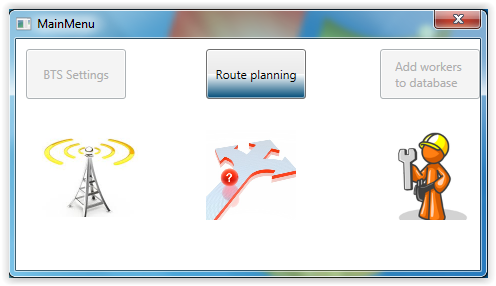
\includegraphics[scale=1]{Pictures/MainMenuUser.png}
\label{fig: MainMenuUser}
\caption{Funkcje dostępne w głównym menu dla serwisanta}{Źródło: opracowanie własne}
\end{figure}
\newpage
Okienko zarządzania stacjami bazowymi jest aktywne tylko dla użytkownika z~prawami administratora. Na rys.~4.7 przedstawiono sposób znalezienia oraz dodania miejscowości do bazy danych. W~przykładzie w~odpowiednim polu wpisano nazwę miasta --- Świdnica, a~następnie kliknięto przycisk \textit{Search for location}. Aplikacja znalazła odpowiednie powiązania, które zostały wyświetlone w~tabeli poniżej. Zaznaczenie miejscowości, a~następnie kliknięcie na przycisk \textit{Add location to database} skutkuje zapisaniem miejscowości w~bazie danych. 

\begin{figure}[!bht]
\centering
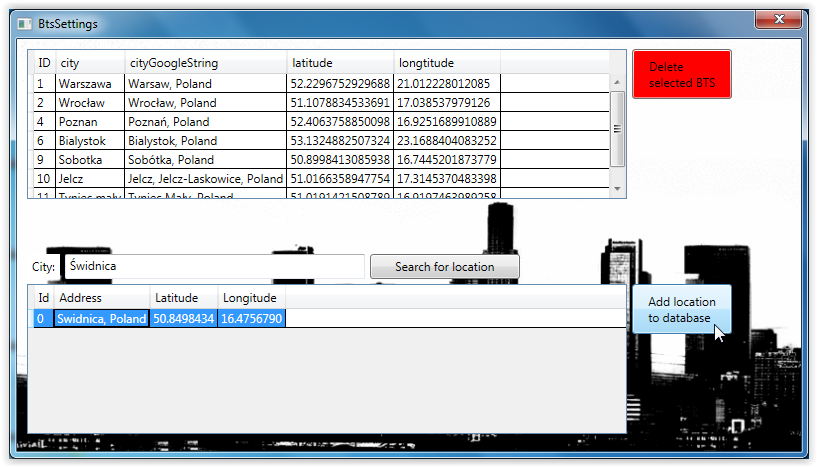
\includegraphics[scale=0.5]{Pictures/AddBTS.png}
\label{fig: AddBTS}
\caption{Znalezienie i dodanie miejscowości}{Źródło: opracowanie własne}
\end{figure}

Na rys.~4.8 można przekonać się o tym, że Świdnica faktycznie została dodana do bazy danych. W~górnej tabeli pod numerem ID równym dwanaście znajduje się wspomniana miejscowość.

\begin{figure}[!bht]
\centering
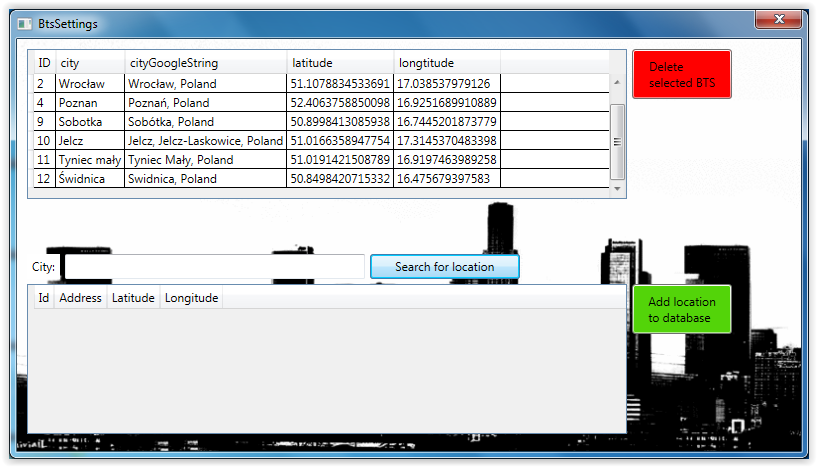
\includegraphics[scale=0.5]{Pictures/AddedCity.png}
\label{fig: AddedCity}
\caption{Dodana miejscowość}{Źródło: opracowanie własne}
\end{figure}
\newpage
Administrator nie tyko jest zobowiązany do dodawania stacji bazowych do bazy danych, ale także do utrzymania należytego porządku, dlatego też czasami trzeba jakąś miejscowość usunąć. Na rys.~4.9 przedstawiono sytuację, w~której firma rezygnuje ze świadczenia usług w~Białymstoku. Zaznaczenie wspomnianej miejscowości, a~następnie kliknięcie przycisku \textit{Delete selected BTS}, powoduje usunięcie lokacji z~bazy danych. Co ciekawe na tym samym rysunku zaprezentowano sytuację, w~której wyszukiwarka zwraca więcej niż jeden wynik (dla hasła Berlin zwrócono stolicę Niemiec oraz cztery miejscowości w~Stanach Zjednoczonych).

\begin{figure}[!bht]
\centering
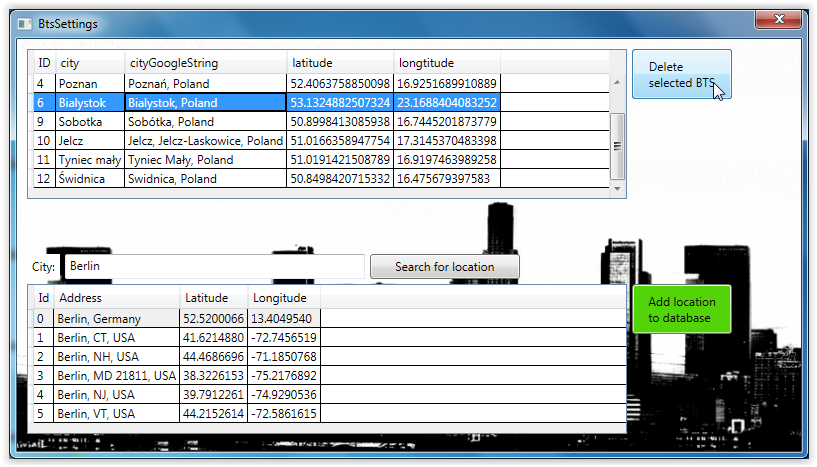
\includegraphics[scale=0.5]{Pictures/DeleteBTE.png}
\label{fig: DeleteBTS}
\caption{Usunięcie lokacji z BTSem}{Źródło: opracowanie własne}
\end{figure}

Aplikacja nie wspiera usuwania, a~także dodawania, wielu lokacji za jednym razem. Zaznaczenie kilku miejscowości, a~następnie kliknięcie przycisku \textit{Delete selected BTS} zakończy się wyświetleniem stosownego komunikatu o~błędzie.  

\begin{figure}[!bht]
\centering
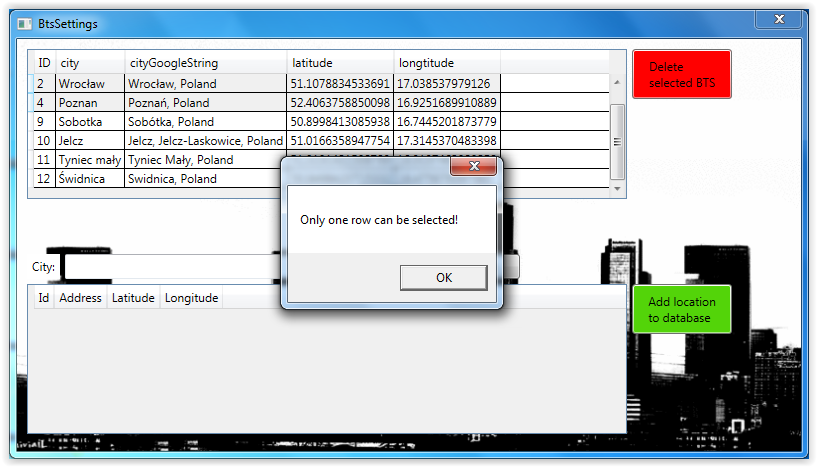
\includegraphics[scale=0.5]{Pictures/OneRowSelected.png}
\label{fig: OneRowSelected}
\caption{Błąd wynikający z zaznaczenia więcej niż jednej pozycji w tabeli}{Źródło: opracowanie własne}
\end{figure}
\newpage
Na rys.~4.11 przedstawiono okno planowania trasy. Z~okna tego może korzystać zarówno administrator jak i~serwisant. W~tabeli po lewej stronie znajdują się miasta dostępne w~bazie danych, po prawej --- miasta, które należy odwiedzić. Przekazywanie lokacji pomiędzy tabeli odbywa się za pomocą przycisków \textit{>>} praz \textit{<<}, co zostało dokładnie opisane w~rozdziale 3. W~przedstawionym przykładzie użytkownik planuje odwiedzić kilka stacji bazowych na Dolnym Śląsku. Wybrano pięć miast: Wrocław, Sobótkę, Jelcz--Laskowice, Tyniec Mały oraz Świdnicę. Kliknięcie przycisku \textit{Start planning!} rozpocznie procedurę wyznaczania najlepszej trasy.

\begin{figure}[!bht]
\centering
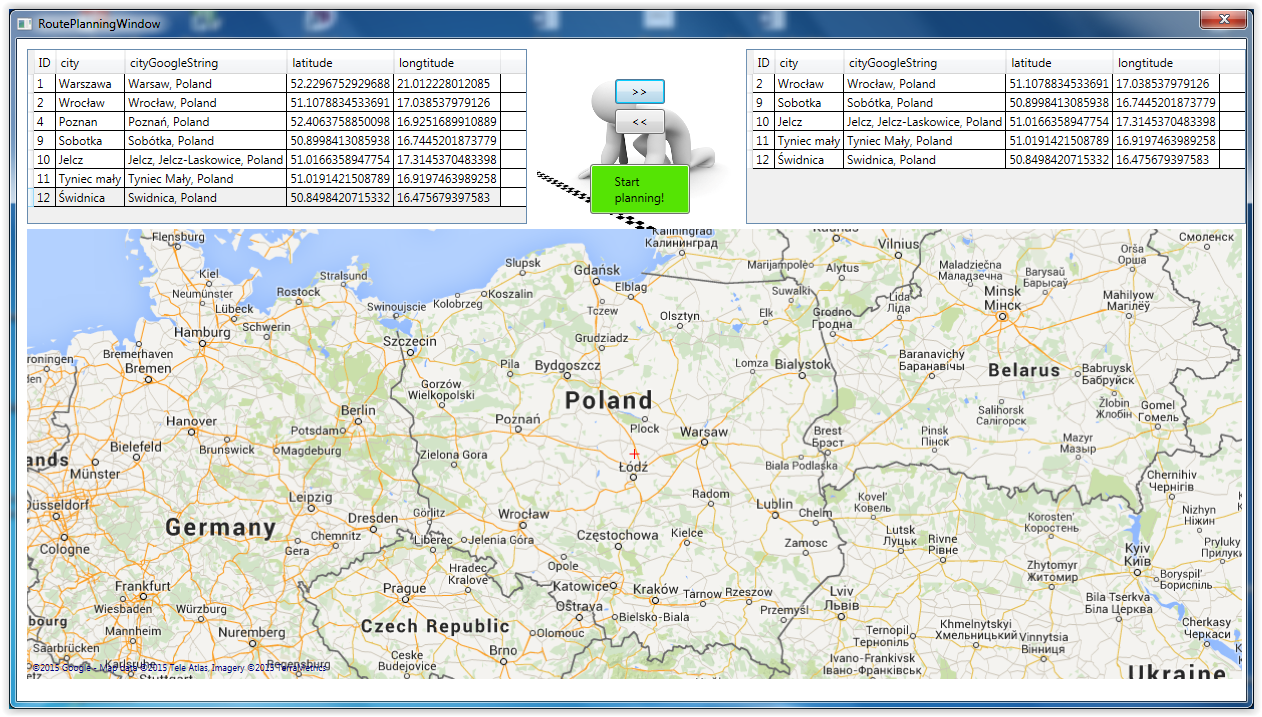
\includegraphics[scale=0.35]{Pictures/ChoosenCities.png}
\label{fig: ChoosenCities}
\caption{Wybór miast do odwiedzenia przez serwisanta}{Źródło: opracowanie własne}
\end{figure}

Po zakończeniu działania procedury rozwiązujące problem komiwojażera program zwraca optymalną trasę (rys.~4.12). Jak widać najlepsza kolejność, w~sensie najkrótszej drogi, dla wskazanych miast jest następująca: Wrocław $\rightarrow$ Jelcz--Laskowice $\rightarrow$ Tyniec Mały $\rightarrow$ Świdnica $\rightarrow$ Sobótka $\rightarrow$ Wrocław. Serwisant podczas odwiedzania wskazanych lokacji przejedzie trasę wynoszącą 162,2 km. Kliknięcie przycisku \textit{OK} zamyka aktualne okno.

\begin{figure}[!bht]
\centering
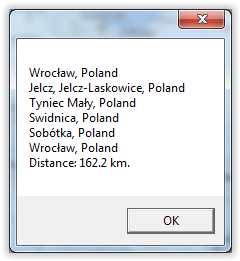
\includegraphics[scale=1]{Pictures/OptimalRoute.png}
\label{fig: OptimalRoute}
\caption{Przedstawienie optymalnej trasy}{Źródło: opracowanie własne}
\end{figure}
\newpage
Na rys.~4.13 przedstawiono wyrysowaną optymalną, wyznaczoną przez program trasę dla wskazanych miast. W~tym przypadku należy mieć na uwadze ograniczenia aplikacji wspomniane w~rozdziale 3. 

\begin{figure}[!bht]
\centering
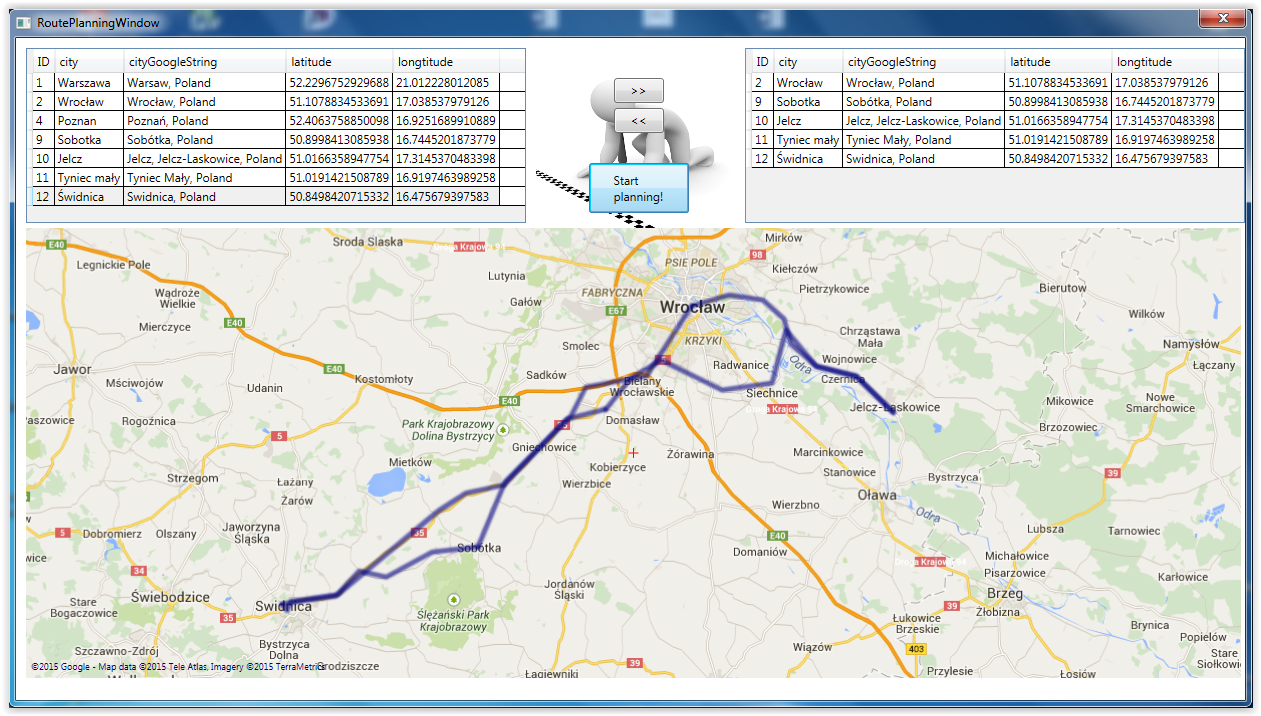
\includegraphics[scale=0.35]{Pictures/DrawedRoute.png}
\label{fig: DrawedRoute}
\caption{Optymalna trasa}{Źródło: opracowanie własne}
\end{figure}
\newpage
Rysunek 4.14 przedstawia okno zarządzania pracownikami, które dostępne jest tylko dla użytkownika z~uprawnieniami administratora. W~podanym przykładzie administrator wprowadził nowego serwisanta (poprzez podanie jego loginu i~hasła oraz kliknięcie przycisku \textit{Add user}). Niestety pomylił się i~przyznał mu prawa administratora.

\begin{figure}[!bht]
\centering
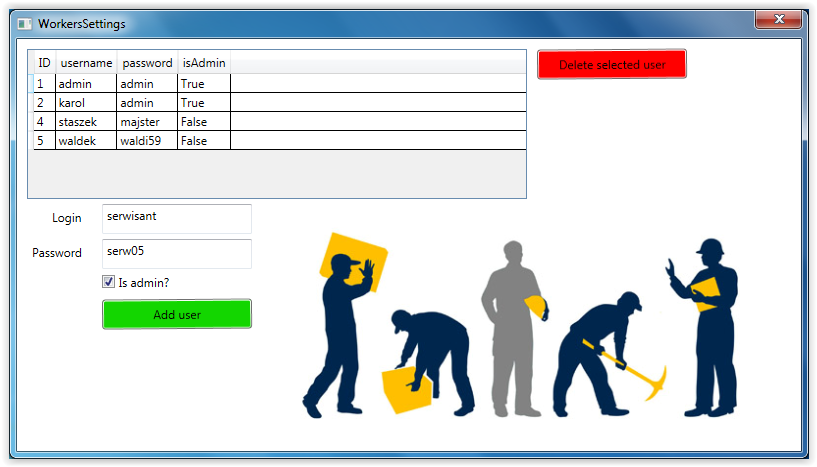
\includegraphics[scale=0.5]{Pictures/AddAdmin.png}
\label{fig: AddAdmin}
\caption{Dodanie serwisanta z błędnymi uprawnieniami}{Źródło: opracowanie własne}
\end{figure}

W~celu naprawienia zaistniałej pomyłki administrator zaznacza odpowiedni rekord w~bazie danych, a~następnie klika przycisk \textit{Delete selected user} (rys.~4.15).

\begin{figure}[!bht]
\centering
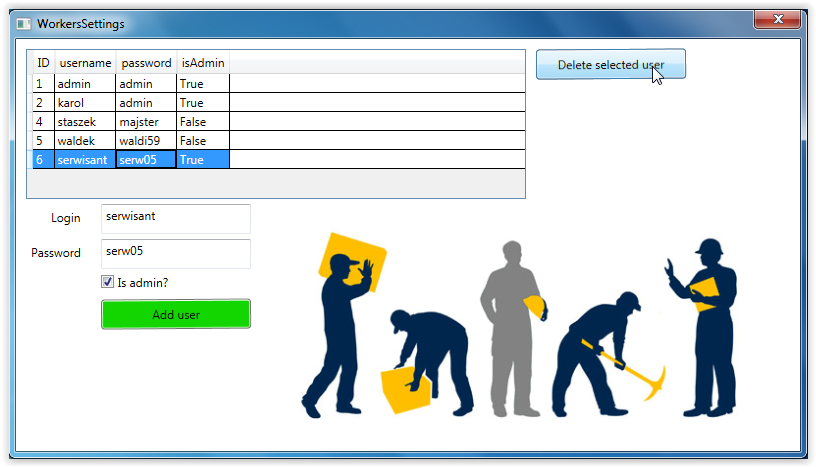
\includegraphics[scale=0.5]{Pictures/DeletedUser.png}
\label{fig: DeletedUser}
\caption{Usunięcie błędnie dodanego serwisanta}{Źródło: opracowanie własne}
\end{figure}

Na rys.~4.16 widać, że serwisant z~prawami administratora został usunięty, a~dodano nowego pracownika, który nie będzie mógł już zarządzać stacjami bazowymi oraz innymi użytkownikami aplikacji.

\begin{figure}[!bht]
\centering
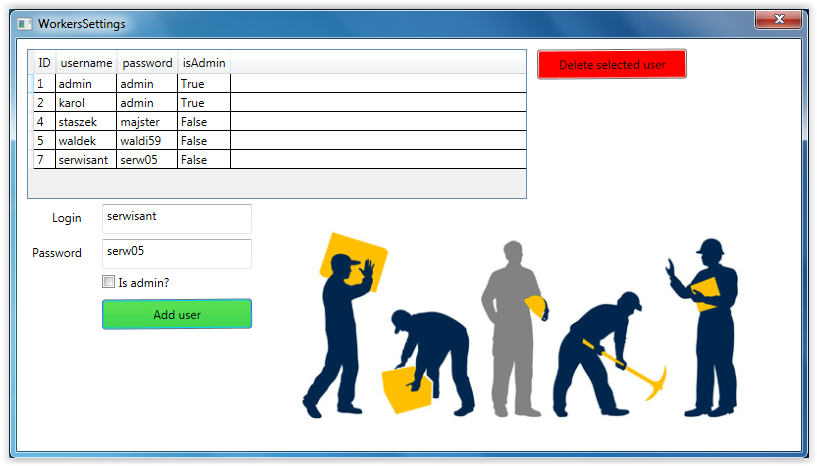
\includegraphics[scale=0.5]{Pictures/AddedCorrectUser.png}
\label{fig: AddedCorrectUser}
\caption{Dodanie serwisanta z poprawnymi uprawnieniami}{Źródło: opracowanie własne}
\end{figure}
\newpage
W trosce o~bezpieczeństwo pracowników wprowadzono w~aplikacji odpowiednie ulepszenia, które zapewnią jak najlepsze warunki pracy serwisantów. Uwzględniając niezbyt pochlebna reputację Sosnowca dojazd tam jest niemożliwy (rys.~4.17).

\begin{figure}[!bht]
\centering
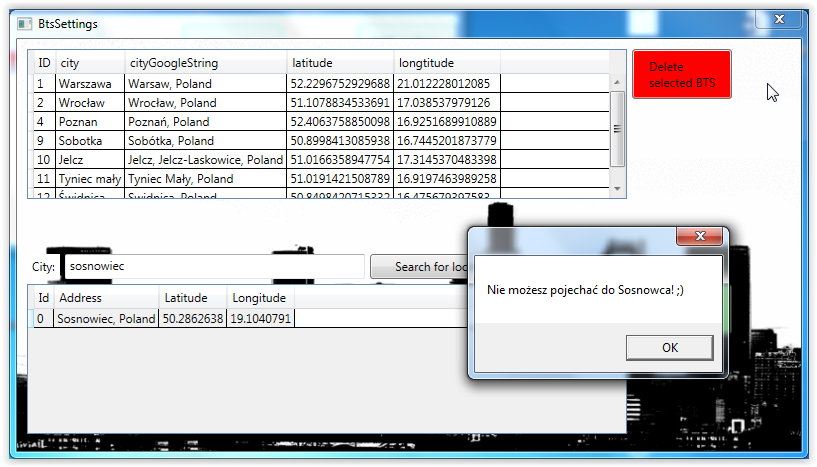
\includegraphics[scale=0.5]{Pictures/Sosnowiec.png}
\label{fig: Sosnowiec}
\caption{Błędne wskazanie miejscowości --- Sosnowiec}{Źródło: opracowanie własne}
\end{figure}

Podobnie jak w~przypadku Sosnowca nie jest także możliwy wyjazd do Radomia (rys.~4.18).

\begin{figure}[!bht]
\centering
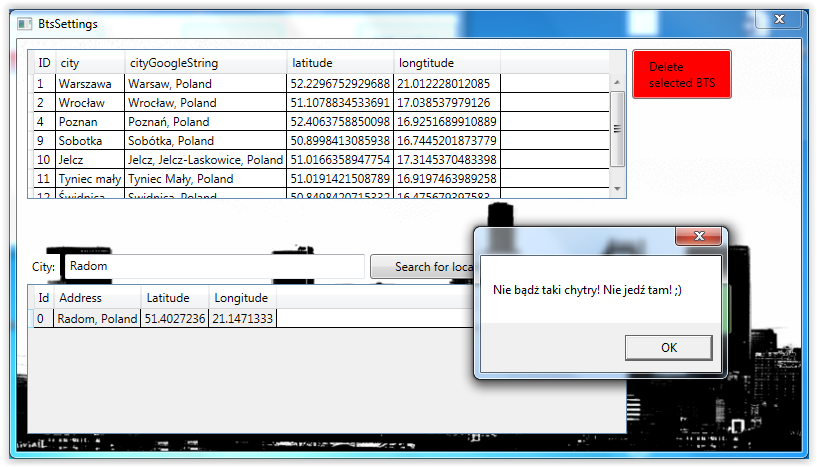
\includegraphics[scale=0.5]{Pictures/Radom.png}
\label{fig: Radom}
\caption{Błędne wskazanie miejscowości --- Radom}{Źródło: opracowanie własne}
\end{figure}
\newpage
Niniejsza prezentacja działania programu powinna utwierdzić w~przekonaniu, że zaprojektowana aplikacja jest skutecznym narzędziem pozwalającym planować trasę dla serwisanta stacji bazowych.

\chapter{Zakończenie}
W ramach niniejszego projektu wykonano kompleksową aplikację, która ma zastosowanie praktyczne. Dzięki zaprojektowanemu programowi możliwe jest wyznaczenie optymalnej trasy dla serwisanta firmy telekomunikacyjnej, którego obowiązkiem jest konserwacja stacji bazowych w~różnych miejscowościach. Przedstawione zagadnienie jest rzeczywistą realizacją znanego w~literaturze specjalistycznej problemu komiwojażera.

Aplikacja została napisana w~języku programowania C Sharp. Wykorzystano również wiele narzędzi dostarczonych przez firmę Microsoft, które pozwalają na skonstruowanie zaawansowanego interfejsu graficznego. Wśród zastosowanych narzędzi wymienić należy: Microsoft Visual Studio, platforma .NET, GMap.NET, Microsoft Blend, Windows Presentation Foundation.

Poza interfejs graficznym zaimplementowano także algorytm komiwojażera, który wyznacza optymalną trasę dla małych grafów. Założenie taki jest sensowne, gdyż serwisant nie jest w~stanie odwiedzić w~ciągu dnia zbyt dużej liczby miejscowości. 

Całość aplikacji wzbogaca baza danych zrealizowana w~aplikacji SQL Server Management Studio 2008. Dzięki zastosowaniu języka C Sharp połączenie z~bazą danych jest proste i~intuicyjne poprzez zastosowanie technologii LINQ.

W~ramach niniejszej dokumentacji projektu zaprezentowano również rozbudowany przykład praktyczny, który przedstawia funkcjonalności aplikacji oraz sposób jej użycia. Przybliżono również zastosowane narzędzia, oprogramowanie oraz algorytm.

\clearpage
\phantomsection
\addcontentsline{toc}{chapter}{Bibliografia}
\begin{thebibliography}{99}

\bibitem{GMap} \textit{GMap.NET --- Great Maps for Windows Forms $\&$ Presentation}. Dostępny na: \url{https://greatmaps.codeplex.com/} (dostęp: 29.03.2015~r.).

\bibitem{TSP_Tarnow} \textit{Problem komiwojażera}. Dostępny na: \url{http://edu.i-lo.tarnow.pl/inf/alg/001_search/0140.php} (dostęp: 29.03.2015~r.).

\bibitem{TSP_Wiki} \textit{Travelling salesman problem}. Dostępny na: \url{http://en.wikipedia.org/wiki/Travelling_salesman_problem} (dostęp: 29.03.2015~r.).

\end{thebibliography}

\clearpage
\phantomsection
\addcontentsline{toc}{chapter}{Spis rysunków}
\listoffigures

\end{document}
